\chapter{Background}
\label{chap:background}

\section{Definitions and vocabulary}
\label{sec:background_definitions}

\subsection*{Identity}
A set of attributes that identifies an entity~\cite{Weik2001}. An entity can be a system, process or individual, but identity in this paper will exclusively reference a persons identity if not explicitly stated otherwise. 
\subsection*{Identity Owner}
The owner of the digital identity, also known as the user.

\subsection*{Identity Provider}
An entity that verifies and signs attributes associated with an identity to provide a certain level of trust in the validity of the information. This could be governmental bodies, banks and other entities that service providers trust.

\subsection*{Service Provider}
An entity that provide some sort of service, and in this context is reliant on a knowing some information relating to the identity of the user. An example of this could be a gambling website ensuring their users are over 18 years of age.

\subsection*{Claims}
Attributes a user or identity owner presents to a service provider 

\section{Distributed Ledgers}
Distributed Ledger Technology (DLT) is a collective term for a immutable ledger that is replicated and synchronized over a large number of nodes where additions to the ledger is agreed upon by consensus in the network. The main advantage of DLTs is the absence of central administrators and data storage, eliminating the need for a trusted third party. The most known type of DLT is blockchain, but in the last few years another approach using Directed Acyclic Graphs (DAG) has been ustilized. Both technologies are explained in detail below.

\label{sec:background_dlt}
\subsection{Blockchain}
Bitcoin was the first application of a blockchain, and is based on a proof-of-work system to represent a majority decision. The miners collect pending transactions in the network and form potential blocks, illustrated in Figure \ref{fig:blockchain}, and then, hash the contents of this block with an variable nonce to meet a certain criteria~\cite{bitcoin2008}. For Bitcoin this criteria is that the hash must begin with a certain number of zeros, and this number of zeros can be increased or decreased to compensate for variable computational power in the network~\cite{bitcoin2008}. The complexity is varied to maintain a block creation rate of around one block per 10 minutes, but the nature of the psudorandomization of hashing algorithms makes this vary greatly. As long as the majority of computational power is controlled by nodes not trying to attack the network, the blockchain serves as a ledger of witnessed transactions with proved ownership.

\begin{figure}[ht]
    \centering
    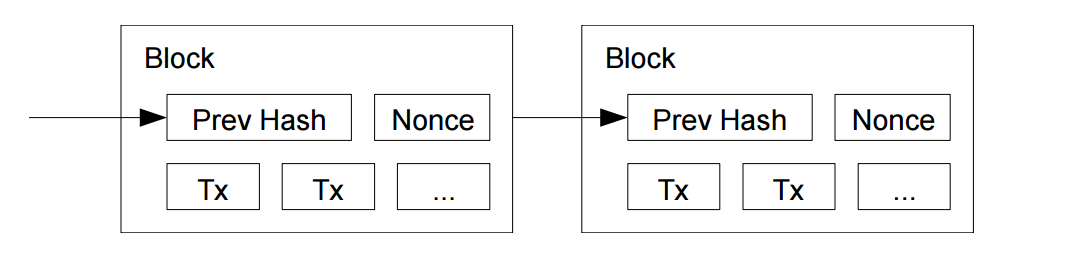
\includegraphics[width=1\textwidth]{blockchain}
    \caption{Visualization of blockchain \cite{bitcoin2008}}
    \label{fig:blockchain}
\end{figure}

After the success of Bitcoin, hundreds of other currencies has been introduced with variations and improvements to most aspects of the original technology. One of the big variations from the original technology is Proof-of-Stake as an alternative to Proof-of-Work, which in its essence is consensus reach based on majority stake voting. A nodes vote is weighed with the stake, or number of coins, the node owns - the argument being the more you own, the less likely you are to try to undermine the value of your own investment. The main advantage of Proof-of-Stake is that it is theoretically faster and requires considerably less computational resources. 

With the growing success of cryptocurrency, or crypto tokens, the incentive for miners has increased with the price. \cite{VRANKEN20171} estimates the total power consumption to be between 100 and 500 MW, the equivalent of a small nation state, and the inefficiency of the Proof-of-Work (PoW) has made Proof-of-Stake (PoS) look like a strong candidate. In the later years, several PoS currencies has been proposed and launched~\cite{Li2017,nxt_whitepaper,blackcoin_pos} but have yet to achieve large market adoption.  PoS implementations sill suffer from some major security concerns, and proposed attacks like~\textit{nothing at stake} and~\textit{long-range attacks} is probably holding the adoption back~\cite{Li2017}.

\subsection{Directed Acyclic Graphs }

Directed Acyclic Graph (DAG), here based on the tangle implementation in IOTA~\cite{IOTA_Whitepaper}. The transactions are theoretically instant and without traditional fees, and are designed to scale infinitely. The tangle is based on a Directed Acyclic Graph (DAG) rather than a traditional chain of blocks, where each transaction is stored separately in the graph, illustrated in Figure~\ref{fig:tangle}. To make a transaction on the IOTA network, the issuing party must approve two previous transactions effectivly doing the Proof-of-Work. This is the basis for the free transactions, as no miner is compensated.

One of the main concerns around a DAC based approach is the succession of transactions. In a regular blockchain, the block number clearly states what order transactions occurred, while in a DAC it can be impossible to determine the order of two transactions with respect to time.

\begin{figure}[ht]
    \centering
    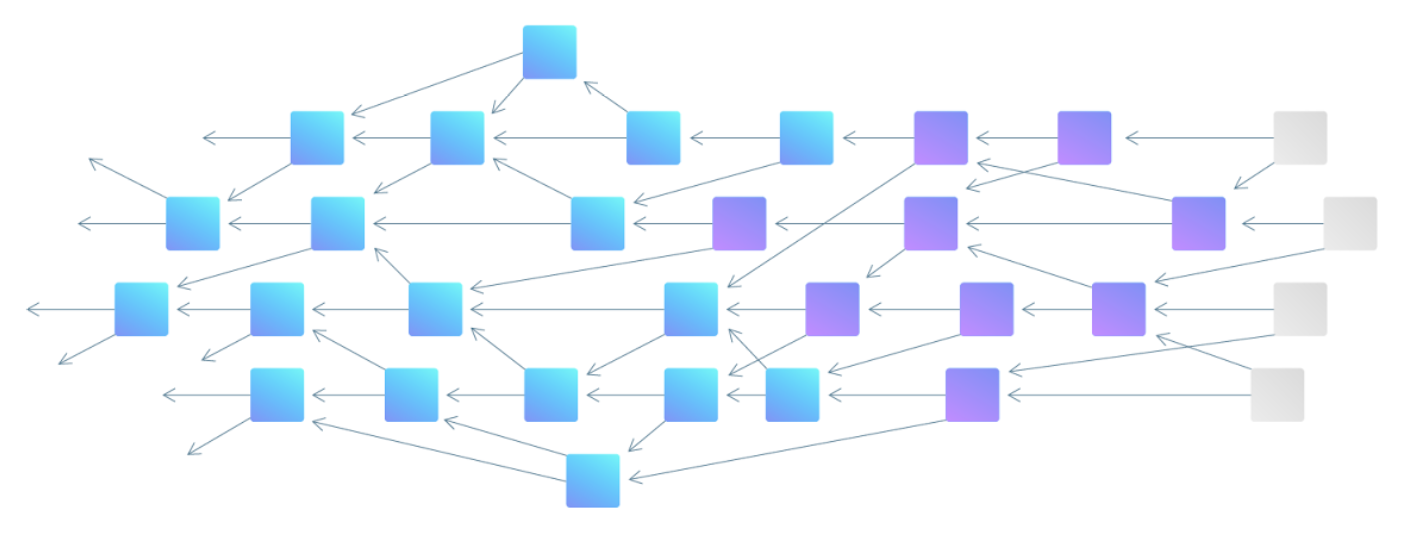
\includegraphics[width=1\textwidth]{tangle}
    \caption{Visualization of the tangle \cite{IOTA_Whitepaper}}
    \label{fig:tangle}
\end{figure}


\section{Traditional Identity Systems}
The most common user management in online services today is still the traditional localized register of users where the user has to sign up with their information directly on the website. This poses several challenges for both the user and the service provider. For the user, this often forces them to either use the same password on several services, or manage a increasingly large number of passwords. The number of online services an average person uses today, having different passwords for each is a daunting task, often eliminating this option. If the user uses the same password everywhere, chances are one of those services uses bad practices and the password is leaked and the adversary can access all the users accounts using the same password. For the service provider, the users are trusting them with personal information that they have to manage and protect responsibly.

The second most used method is federated identities, where the user trusts one identity provider and registers with them. The user can then log in to several services using the same account. Most known applications of this is seen on websites that has the option "Sign in with Facebook/Google". This also poses some challenges; the user rely on one provider to store and protect their data, and also facilitating for tracking and big data gathering as that provider will get information on what services the user is accessing when.

\section{Web-of-trust}
The web of trust is a public-key authentication system originally built on PGP. A user can build confidence in their identity by having other users sign their public key~\cite{Azouvi2017}. In an identity management system where we distinguish between Users and Service Providers, we can build on this idea. We can look at a scenario where a User has their identity verified and signed by visiting the governmental department issuing passports for their citizens. If the user wants proof that they also have a drivers license, and the issuing body (DMV, Statens Vegvesen, e.g.) trusts that department, they can link a drivers license to that identity based on the verified identity already in the ledger. This opens up for possibilities where the User can visit a small number of Identity Providers and establish a base identity, and then build upon that over the internet.


\section{Self-Sovereign Identity (SSI)}
When Self-Sovereign Identity (SSI) is used as a term within this paper, if references a model of identity management that ensures that the user fully owns and controls their own data. This also includes who has access to the attributes and the possibility to add, delete or revoke these attributes at their own discretion. To assure the privacy required by a SSI-model, the attributes must be stored and processed in a secure manner, and segregation of attributes such that anyone other than the owner can connect the different attributes to the identity. The identity must be maintained and stored without a federation or third party control, and is therefor reliant on a distributed and truly decentralized system.

Even though EGIZ Whitepaper on Self-Sovereign Identity~\cite{ssi} states that a requirement for a self-sovereign identity model is that access to the information is logged. This is a trade-off between privacy and security and is discussed further in INSERT CHAPTER HERE. The definition which this thesis will rely on is Christopher Allen's principles of self-sovereign identity. One principle that Christopher Allen does not explicitly mention is cost, but the principle of \textit{Interoperability} states that an identity must be \textit{widely available} and this thesis will assume that to be widely available, it must be free. 

The following list is the ten principles of self-sovereign identity as described by Christopher Allen~\cite{SSIPrinciples}:

\subsection{Existence} \textit{Users must have an independent existence.} Any self-sovereign identity is ultimately based on the ineffable “I” that’s at the heart of identity. It can never exist wholly in digital form. This must be the kernel of self that is upheld and supported. A self-sovereign identity simply makes public and accessible some limited aspects of the “I” that already exists.
\subsection{Control} \textit{Users must control their identities.} Subject to well-understood and secure algorithms that ensure the continued validity of an identity and its claims, the user is the ultimate authority on their identity. They should always be able to refer to it, update it, or even hide it. They must be able to choose celebrity or privacy as they prefer. This doesn’t mean that a user controls all of the claims on their identity: other users may make claims about a user, but they should not be central to the identity itself.
\subsection{Access} \textit{Users must have access to their own data.} A user must always be able to easily retrieve all the claims and other data within his identity. There must be no hidden data and no gatekeepers. This does not mean that a user can necessarily modify all the claims associated with his identity, but it does mean they should be aware of them. It also does not mean that users have equal access to others’ data, only to their own.
\subsection{Transparency} \textit{Systems and algorithms must be transparent.} The systems used to administer and operate a network of identities must be open, both in how they function and in how they are managed and updated. The algorithms should be free, open-source, well-known, and as independent as possible of any particular architecture; anyone should be able to examine how they work.
\subsection{Persistence} \textit{Identities must be long-lived.} Preferably, identities should last forever, or at least for as long as the user wishes. Though private keys might need to be rotated and data might need to be changed, the identity remains. In the fast-moving world of the Internet, this goal may not be entirely reasonable, so at the least identities should last until they’ve been outdated by newer identity systems. This must not contradict a “right to be forgotten”; a user should be able to dispose of an identity if he wishes and claims should be modified or removed as appropriate over time. To do this requires a firm separation between an identity and its claims: they can't be tied forever.
\subsection{Portability} \textit{Information and services about identity must be transportable.} Identities must not be held by a singular third-party entity, even if it's a trusted entity that is expected to work in the best interest of the user. The problem is that entities can disappear — and on the Internet, most eventually do. Regimes may change, users may move to different jurisdictions. Transportable identities ensure that the user remains in control of his identity no matter what, and can also improve an identity’s persistence over time.
\subsection{Interoperability} \textit{Identities should be as widely usable as possible.} Identities are of little value if they only work in limited niches. The goal of a 21st-century digital identity system is to make identity information widely available, crossing international boundaries to create global identities, without losing user control. Thanks to persistence and autonomy these widely available identities can then become continually available.
\subsection{Consent} \textit{Users must agree to the use of their identity.} Any identity system is built around sharing that identity and its claims, and an interoperable system increases the amount of sharing that occurs. However, sharing of data must only occur with the consent of the user. Though other users such as an employer, a credit bureau, or a friend might present claims, the user must still offer consent for them to become valid. Note that this consent might not be interactive, but it must still be deliberate and well-understood.
\subsection{Minimalization} \textit{Disclosure of claims must be minimized.} When data is disclosed, that disclosure should involve the minimum amount of data necessary to accomplish the task at hand. For example, if only a minimum age is called for, then the exact age should not be disclosed, and if only an age is requested, then the more precise date of birth should not be disclosed. This principle can be supported with selective disclosure, range proofs, and other zero-knowledge techniques, but non-correlatibility is still a very hard (perhaps impossible) task; the best we can do is to use minimalization to support privacy as best as possible.
\subsection{Protection} \textit{The rights of users must be protected.} When there is a conflict between the needs of the identity network and the rights of individual users, then the network should err on the side of preserving the freedoms and rights of the individuals over the needs of the network. To ensure this, identity authentication must occur through independent algorithms that are censorship-resistant and force-resilient and that are run in a decentralized manner.


\section{Available Self-Sovereign Identity Systems}
\label{sec:ssi_systems}
\subsection{Sovrin}
The Sovrin Foundation have set out on a mission to standardize and create an infrastructure for Self-Sovereign identities, using blockchain as storage for Distributed Identities such that anyone can issue or verify it~\cite{sovrin}. The Sovrin blockchain has been designed only for identity, and is taking steps to move the digital trust away from centralized CAs to a web of trust model. The Soverin SSI model is not dependent on any particular distributed ledger, but can work with any blockchain that meets the fundamental principles. Sovrin has implemented their identity system in a specific instantiation of Hyperledger's Indy project.
\\\\
https://sovrin.org/wp-content/uploads/Sovrin-Protocol-and-Token-White-Paper.pdf
\\\\ https://sovrin.org/wp-content/uploads/2017/04/The-Technical-Foundations-of-Sovrin.pdf
\\\\
https://www.evernym.com/solution/
https://www.evernym.com/

\subsection{uPort}
https://whitepaper.uport.me/uPort\_whitepaper\_DRAFT20170221.pdf


\subsection{Civic}
https://www.civic.com/

\subsection{Comparison}
\begin{table}[ht]
\begin{center}
\begin{tabular}{|l|c|c|c|}
\hline
 & Sovrin & uPort & Civic \\
\hline
Minable & No & Yes & Yes  \\
Attribute Segregation & Yes & Yes & Yes \\
Storage & On-Chain & Off-Chain & On-Device \\
Smart Contracts & No & Yes & Yes \\
Key Management & DPKI & DPKI & Ethereum Addresses \\
Verification & Permissioned & Permissionless & Permissionless  \\
\hline
\end{tabular}
\caption[Comparison of SSI Systems]{Tabular comparison of Self-Sovereign Identity Systems currently available}
\label{tbl:SSIS}
\end{center}
\end{table}